\documentclass[12pt]{article}
\usepackage{amsmath}
\usepackage{amssymb}
\usepackage{graphicx}
\usepackage{tcolorbox}
\usepackage{enumitem}
\usepackage{geometry}
\usepackage{xcolor}
\usepackage{tikz}
\usetikzlibrary{angles,quotes}

% Custom colors
\definecolor{primary}{RGB}{41, 128, 185}
\definecolor{secondary}{RGB}{52, 152, 219}
\definecolor{accent}{RGB}{231, 76, 60}
\definecolor{lightgray}{RGB}{236, 240, 241}

% Page setup
\geometry{a4paper, margin=1in}

% Title page info
\title{Pre-Calculus 11 \\ Chapter 3: Trigonometry}
\author{Created by Yi-Chen Lin}
\date{\today}

\begin{document}

\maketitle

\section*{Chapter Overview}
This chapter covers the fundamentals of trigonometry, including:
\begin{itemize}
    \item Basic trigonometric functions and ratios
    \item Angles in standard position
    \item Special triangles and exact values
    \item Solving angles in all four quadrants
    \item Sine Law and its ambiguous case
    \item Cosine Law
\end{itemize}

\section{3.1 Basic Trigonometric Functions}
\subsection*{Key Concepts}
\begin{tcolorbox}[colback=lightgray,colframe=primary,title=Trig Ratios]
    \begin{itemize}
        \item $\sin\theta = \frac{\text{Opposite}}{\text{Hypotenuse}}$
        \item $\cos\theta = \frac{\text{Adjacent}}{\text{Hypotenuse}}$
        \item $\tan\theta = \frac{\text{Opposite}}{\text{Adjacent}}$
        \item Pythagorean Theorem: $a^2 + b^2 = c^2$
    \end{itemize}
\end{tcolorbox}

\subsection*{Diagram}
\begin{center}
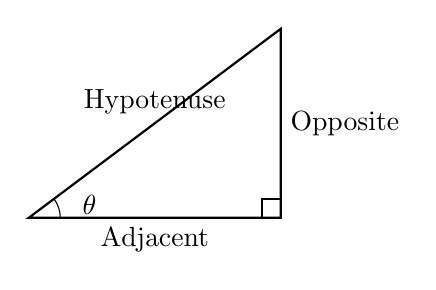
\begin{tikzpicture}[scale=0.8]
    \draw[thick] (0,0) -- (4,0) -- (4,3) -- cycle;
    \draw[thick] (3.7,0) -- (3.7,0.3) -- (4,0.3);
    \node[right] at (4,1.5) {Opposite};
    \node[below] at (2,0) {Adjacent};
    \node[above, sloped] at (2,1.5) {Hypotenuse};
    \draw (0.5,0) arc (0:36.87:0.5);
    \node[right] at (0.7,0.2) {$\theta$};
\end{tikzpicture}
\end{center}

\section{3.2 Angles in Standard Position}
\subsection*{Key Concepts}
\begin{tcolorbox}[colback=lightgray,colframe=primary,title=Standard Position]
    \begin{itemize}
        \item Angles measured from the positive $x$-axis
        \item Quadrants I-IV
        \item Reference angle: always positive, between terminal arm and $x$-axis
    \end{itemize}
\end{tcolorbox}

\subsection*{Diagram}
\begin{center}
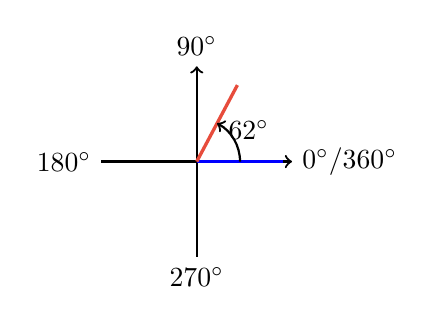
\begin{tikzpicture}[scale=1.1]
    \draw[thick,->] (-1.1,0) -- (1.1,0) node[right] {$0^\circ$/$360^\circ$};
    \draw[thick,->] (0,-1.1) -- (0,1.1) node[above] {$90^\circ$};
    \draw[thick] (-1,0) -- (-1.1,0) node[left] {$180^\circ$};
    \draw[thick] (0,-1) -- (0,-1.1) node[below] {$270^\circ$};
    \draw[very thick,blue] (0,0) -- (1,0);
    \draw[very thick,accent] (0,0) -- ({cos(62)},{sin(62)});
    \draw[->,thick] (0.5,0) arc (0:62:0.5);
    \node at ({0.7*cos(31)},{0.7*sin(31)}) {$62^\circ$};
\end{tikzpicture}
\end{center}

\section{3.3 Special Triangles}
\subsection*{Key Concepts}
\begin{tcolorbox}[colback=lightgray,colframe=primary,title=Special Triangles]
    \begin{itemize}
        \item $30^\circ$-$60^\circ$-$90^\circ$ and $45^\circ$-$45^\circ$-$90^\circ$ triangles
        \item Exact values for $\sin$, $\cos$, $\tan$ of special angles
    \end{itemize}
\end{tcolorbox}

\subsection*{Diagrams}
\begin{center}
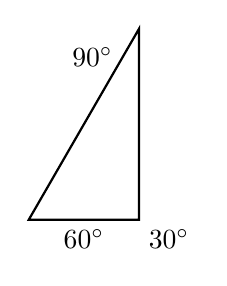
\begin{tikzpicture}[scale=0.7]
    \draw[thick] (0,0) -- (2,0) -- (2,3.464) -- cycle;
    \node[below] at (1,0) {$60^\circ$};
    \node[above left] at (1.7,2.6) {$90^\circ$};
    \node[below right] at (2,0) {$30^\circ$};
\end{tikzpicture}
\hspace{2cm}
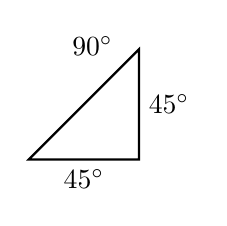
\begin{tikzpicture}[scale=0.7]
    \draw[thick] (0,0) -- (2,0) -- (2,2) -- cycle;
    \node[below] at (1,0) {$45^\circ$};
    \node[right] at (2,1) {$45^\circ$};
    \node[above left] at (1.7,1.7) {$90^\circ$};
\end{tikzpicture}
\end{center}

\section{3.4 Solving Angles in All Four Quadrants}
\subsection*{Key Concepts}
\begin{tcolorbox}[colback=lightgray,colframe=primary,title=Quadrant Rules]
    \begin{itemize}
        \item ASTC rule: All Students Take Calculus (signs of trig functions in each quadrant)
        \item Reference angle method for finding all solutions
    \end{itemize}
\end{tcolorbox}

\subsection*{Diagram}
\begin{center}
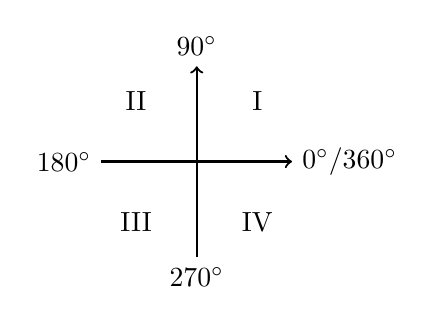
\begin{tikzpicture}[scale=1.1]
    \draw[thick,->] (-1.1,0) -- (1.1,0) node[right] {$0^\circ$/$360^\circ$};
    \draw[thick,->] (0,-1.1) -- (0,1.1) node[above] {$90^\circ$};
    \draw[thick] (-1,0) -- (-1.1,0) node[left] {$180^\circ$};
    \draw[thick] (0,-1) -- (0,-1.1) node[below] {$270^\circ$};
    \node at (0.7,0.7) {I};
    \node at (-0.7,0.7) {II};
    \node at (-0.7,-0.7) {III};
    \node at (0.7,-0.7) {IV};
\end{tikzpicture}
\end{center}

\section{3.5 Sine Law}
\subsection*{Key Concepts}
\begin{tcolorbox}[colback=lightgray,colframe=primary,title=Sine Law]
    \begin{itemize}
        \item $\frac{a}{\sin A} = \frac{b}{\sin B} = \frac{c}{\sin C}$
        \item Use for non-right triangles when you have an angle and its opposite side
    \end{itemize}
\end{tcolorbox}

\section{3.6 Ambiguous Case of the Sine Law}
\subsection*{Key Concepts}
\begin{tcolorbox}[colback=lightgray,colframe=primary,title=Ambiguous Case (SSA)]
    \begin{itemize}
        \item SSA case: two sides and a non-included angle
        \item May yield 0, 1, or 2 possible triangles
        \item Check for ambiguous case when using Sine Law
    \end{itemize}
\end{tcolorbox}

\section{3.7 Cosine Law}
\subsection*{Key Concepts}
\begin{tcolorbox}[colback=lightgray,colframe=primary,title=Cosine Law]
    \begin{itemize}
        \item $a^2 = b^2 + c^2 - 2bc\cos A$ (and cyclic)
        \item Use for non-right triangles with SAS or SSS
    \end{itemize}
\end{tcolorbox}

\section*{Chapter Summary}
\begin{tcolorbox}[colback=lightgray,colframe=primary,title=Key Takeaways]
    \begin{itemize}
        \item Know all basic trig ratios and how to use SOH-CAH-TOA
        \item Understand reference angles and quadrant rules
        \item Memorize special triangles and exact values
        \item Apply Sine Law and Cosine Law to solve triangles
        \item Always check for the ambiguous case in SSA
    \end{itemize}
\end{tcolorbox}

\end{document} 